\section{Structured Matrices}
In many linear systems, the singular values do not decay rapidly and the matrix has a large (or even full) $\epsilon$-rank. However, it's off-diagonal blocks of $A$ are often low rank. That is, given the matrix $A\in \mathbb{R}^{n\times n}$ with $n$ being a power of 2, then we can decompose $A$ as
\begin{equation*}
A =
\begin{tikzpicture}[baseline=(current bounding box.center),
every left delimiter/.style={xshift=2mm},
every right delimiter/.style={xshift=-2mm}
]
\matrix[matrix of math nodes,         left delimiter={[},
        right delimiter={]},](m){
A_{11} & A_{12} \\
A_{21} & A_{22} \\
};
\draw[dashed] (m-1-1.north east) -- (m-2-1.south east);
\draw[dashed] (m-1-1.south west) -- (m-2-2.north east);
\end{tikzpicture},
\end{equation*}
and the off-diagonal blocks $A_{12}$ and $A_{21}$ are rank $k$ with $k\ll n$. Often this low-rank off-diagonal block structure can be applied recursively, and the new off-diagonal blocks are still rank $k$.

Let's change the notation so that we can do recursive off-diagonal structured matrices. Define the index set $I_i = \{1, 2, \ldots, n\}$. We let $I_2$ and $I_3$ be the first and second halves of $I_1$. That is

\begin{align*}
    I_2 &= \left\{1, \ldots, \frac{n}{2}\right\}\\
    I_3 &= \left\{\frac{n}{2} + 1, \ldots, n\right\}
\end{align*}

Continuing we have a tree structure


\begin{center}
    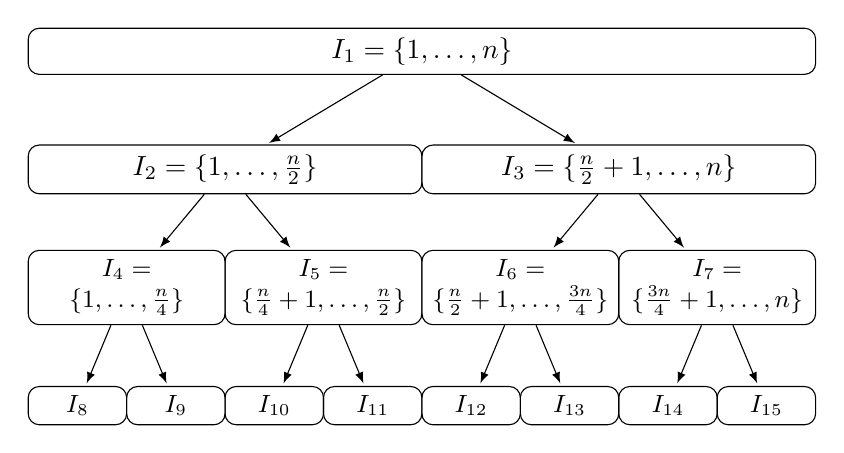
\begin{tikzpicture}[shorten >=1pt,
    edge from parent/.style={draw,-latex},
    level 1/.style={sibling distance=5cm, minimum width=5cm},
    level 2/.style={sibling distance=2.5cm, minimum width=2.5cm,font=\small},
    level 3/.style={sibling distance=1.25cm, minimum width=1.25cm},
    every node/.style = {shape=rectangle, rounded corners,
    draw, align=center}]
    \node[minimum width=10cm](I1){$I_1 = \{1, \ldots, n\}$}
    child {node{$I_2 = \{1, \ldots, \frac{n}{2}\}$}
        child{node{$I_4=$\\$\{1, \ldots, \frac{n}{4}\}$}
            child{node{$I_8$}}
            child{node{$I_9$}}
        }
        child{node{$I_5=$\\$\{\frac{n}{4}+1, \ldots, \frac{n}{2}\}$}
            child{node{$I_{10}$}}
            child{node{$I_{11}$}}
        }
    }
    child {node{$I_3 = \{\frac{n}{2}+1, \ldots, n\}$}
        child{node{$I_6=$\\$\{\frac{n}{2}+1, \ldots, \frac{3n}{4}\}$}
            child{node{$I_{12}$}}
            child{node{$I_{13}$}}
        }
        child{node{$I_7=$\\$\{ \frac{3n}{4}+1, \ldots, n\}$}
            child{node{$I_{14}$}}
            child{node{$I_{15}$}}
        }
    }
    ;
\end{tikzpicture}

\end{center}

Then, for $\sigma, \tau \in \mathbb{N}$ we let $A_{\sigma \tau}$ be the submatrix of $A$ with rows in the index set $I_\sigma$ and columns in the index set $I_\tau$. Then, the new labelling from the above partition is

\begin{equation*}
A =
\begin{tikzpicture}[baseline=(current bounding box.center),
every left delimiter/.style={xshift=2mm},
every right delimiter/.style={xshift=-2mm},
node distance=.5em,
]

\matrix[matrix of math nodes,left delimiter={[},
        right delimiter={]},](m){
A_{22} & A_{23} \\
A_{32} & A_{33} \\
};
\draw[dashed] (m-1-1.north east) -- (m-2-1.south east);
\draw[dashed] (m-1-1.south west) -- (m-2-2.north east);
\node[above = of m-1-1, red]{$I_2$};
\node[above = of m-1-2, red]{$I_3$};
\node[left = of m-1-1, red]{$I_2$};
\node[left = of m-2-1, red]{$I_3$};
\end{tikzpicture}
\end{equation*}

In general
\begin{center}
    \begin{tikzpicture}[decoration=brace]
\matrix[
matrix of math nodes,
nodes in empty cells,
every node/.style = {minimum size=2em},
left delimiter={[},
right delimiter={]},
row sep=.25em,
column sep=1em,
]
(m){
&&\\
&&|[draw, red]| {\color{black} $A_{\sigma\tau}$}\\
&&\\
};
\draw[decorate,transform canvas={yshift=3em},thick, red] (m-2-3.north west) -- node[above=2pt] {$I_{\tau}$} (m-2-3.north east);
\draw[decorate,transform canvas={xshift=-7.5em},thick, red] (m-2-3.south west) -- node[left=2pt] {$I_{\sigma}$} (m-2-3.north west);
\end{tikzpicture}

\end{center}

%% Lecture 23
Applying the off-diagonal structure recursively,
\begin{center}
    \begin{tikzpicture}
    \matrix[
    matrix of math nodes,
    nodes in empty cells,
    left delimiter={[},
    right delimiter={]},
    every node/.style={
        ,
        anchor=center,
        minimum size=3em,
        inner sep=0pt
        },
    ]
    (m)
    {
          $A_{8,   8}$&$A_{8,   9}$&&&&&&\\
          $A_{9,   8}$&$A_{9,   9}$&&&&&&\\
    &&    $A_{10, 10}$&$A_{10, 11}$&&&&\\
    &&    $A_{11, 10}$&$A_{11, 11}$&&&&\\
    &&&&  $A_{12, 12}$&$A_{12, 13}$&&\\
    &&&&  $A_{13, 12}$&$A_{13, 13}$&&\\
    &&&&&&$A_{14, 14}$&$A_{14, 15}$\\
    &&&&&&$A_{15, 14}$&$A_{15, 15}$\\
    };
    \draw[red, dashed] (m-1-1.south west) -- (m-1-2.south east);
    \draw[red, dashed] (m-2-1.south west) -- (m-2-4.south east);
    \draw[red, dashed] (m-3-3.south west) -- (m-3-4.south east);
    \draw[red, dashed] (m-4-1.south west) -- (m-4-8.south east);
    \draw[red, dashed] (m-5-5.south west) -- (m-5-6.south east);
    \draw[red, dashed] (m-6-5.south west) -- (m-6-8.south east);
    \draw[red, dashed] (m-7-7.south west) -- (m-7-8.south east);

    \draw[dashed, red] (m-1-1.north east) -- (m-2-1.south east);
    \draw[dashed, red] (m-1-2.north east) -- (m-4-2.south east);
    \draw[dashed, red] (m-3-3.north east) -- (m-4-3.south east);
    \draw[dashed, red] (m-1-4.north east) -- (m-8-4.south east);
    \draw[dashed, red] (m-5-5.north east) -- (m-6-5.south east);
    \draw[dashed, red] (m-5-6.north east) -- (m-8-6.south east);
    \draw[dashed, red] (m-7-7.north east) -- (m-8-7.south east);
    \node[font=\Large]() at (m-1-3.south east){$A_{4,5}$};
    \node[font=\Large]() at (m-3-1.south east){$A_{5, 4}$};
    \node[font=\Large]() at (m-5-7.south east){$A_{6, 7}$};
    \node[font=\Large]() at (m-7-5.south east){$A_{7, 6}$};
    \node[font=\LARGE]() at (m-2-6.south east){$A_{2, 3}$};
    \node[font=\LARGE]() at (m-6-2.south east){$A_{3, 2}$};
\end{tikzpicture}

\end{center}

If we need to compute $A\vec{x}$, this can be done as follows
\begin{center}
    \begin{tikzpicture}[decoration=brace]
        \matrix[,
    matrix of math nodes,
    nodes in empty cells,
    left delimiter={[},
    right delimiter={]},
    every node/.style={
        %draw,
        font=\tiny,
        anchor=center,
        minimum size=2em,
        inner sep=0pt
        },
    ]
    (m1)
   {
          &&&&&&&\\
          &&&&&&&\\
    &&    &&&&&\\
    &&    &&&&&\\
    &&&&  &&&\\
    &&&&  &&&\\
    &&&&&&&\\
    &&&&&&&\\
    };

    \draw[red, dashed] (m1-4-1.south west) -- (m1-4-8.south east);
    \draw[dashed, red] (m1-1-4.north east) -- (m1-8-4.south east);
    \node[font=\LARGE]() at (m1-2-6.south east){$A_{2, 3}$};
    \node[font=\LARGE]() at (m1-6-2.south east){$A_{3, 2}$};
    \node[font=\LARGE]() at (m1-2-2.south east){$0$};
    \node[font=\LARGE]() at (m1-6-6.south east){$0$};
    \matrix[right =of m1,
    matrix of math nodes,
    nodes in empty cells,
    left delimiter={[},
    right delimiter={]},
    every node/.style={
        %draw,
        font=\tiny,
        anchor=center,
        minimum size=2em,
        inner sep=0pt
        },
    ]
    (m2)
   {
          &&&&&&&\\
          &&&&&&&\\
    &&    &&&&&\\
    &&    &&&&&\\
    &&&&  &&&\\
    &&&&  &&&\\
    &&&&&&&\\
    &&&&&&&\\
    };

    \draw[red, dashed] (m2-4-1.south west) -- (m2-4-8.south east);
    \draw[dashed, red] (m2-1-4.north east) -- (m2-8-4.south east);
    \draw[red, dashed] (m2-2-1.south west) -- (m2-2-4.south east);
    \draw[dashed, red] (m2-1-2.north east) -- (m2-4-2.south east);
    \draw[dashed, red] (m2-5-6.north east) -- (m2-8-6.south east);
    \draw[red, dashed] (m2-6-5.south west) -- (m2-6-8.south east);
    \node[font=\Large]() at (m2-1-3.south east){$A_{4,5}$};
    \node[font=\Large]() at (m2-3-1.south east){$A_{5, 4}$};
    \node[font=\Large]() at (m2-5-7.south east){$A_{6, 7}$};
    \node[font=\Large]() at (m2-7-5.south east){$A_{7, 6}$};
    \node[font=\Large]() at (m2-1-1.south east){$0$};
    \node[font=\Large]() at (m2-3-3.south east){$0$};
    \node[font=\Large]() at (m2-5-5.south east){$0$};
    \node[font=\Large]() at (m2-7-7.south east){$0$};
    \node[font=\LARGE]() at (m2-2-6.south east){$0$};
    \node[font=\LARGE]() at (m2-6-2.south east){$0$};
    \node[right = .75em of m1](){$+$};
    \node[right = .75em of m2](){$+$};


    \matrix[below=of m1,
    matrix of math nodes,
    nodes in empty cells,
    left delimiter={[},
    right delimiter={]},
    every node/.style={
        %draw,
        font=\tiny,
        anchor=center,
        minimum size=2em,
        inner sep=0pt
        },
    ]
    (m3)
        {
          &$A_{8,   9}$&&&&&&\\
          $A_{9,   8}$&&&&&&&\\
    &&    &$A_{10, 11}$&&&&\\
    &&    $A_{11, 10}$&&&&&\\
    &&&&  &$A_{12, 13}$&&\\
    &&&&  $A_{13, 12}$&&&\\
    &&&&&&&$A_{14, 15}$\\
    &&&&&&$A_{15, 14}$&\\
    };
    \draw[red, dashed] (m3-1-1.south west) -- (m3-1-2.south east);
    \draw[red, dashed] (m3-2-1.south west) -- (m3-2-4.south east);
    \draw[red, dashed] (m3-3-3.south west) -- (m3-3-4.south east);
    \draw[red, dashed] (m3-4-1.south west) -- (m3-4-8.south east);
    \draw[red, dashed] (m3-5-5.south west) -- (m3-5-6.south east);
    \draw[red, dashed] (m3-6-5.south west) -- (m3-6-8.south east);
    \draw[red, dashed] (m3-7-7.south west) -- (m3-7-8.south east);

    \draw[dashed, red] (m3-1-1.north east) -- (m3-2-1.south east);
    \draw[dashed, red] (m3-1-2.north east) -- (m3-4-2.south east);
    \draw[dashed, red] (m3-3-3.north east) -- (m3-4-3.south east);
    \draw[dashed, red] (m3-1-4.north east) -- (m3-8-4.south east);
    \draw[dashed, red] (m3-5-5.north east) -- (m3-6-5.south east);
    \draw[dashed, red] (m3-5-6.north east) -- (m3-8-6.south east);
    \draw[dashed, red] (m3-7-7.north east) -- (m3-8-7.south east);
    \node[right = .75em of m3](){$+$};
    \matrix[,
    right=of m3,
    matrix of math nodes,
    nodes in empty cells,
    left delimiter={[},
    right delimiter={]},
    every node/.style={
        %draw,
        font=\tiny,
        anchor=center,
        minimum size=2em,
        inner sep=0pt
        },
    ]
    (m4)
    {
          $A_{8,   8}$&&&&&&&\\
          &$A_{9,   9}$&&&&&&\\
    &&    $A_{10, 10}$&&&&&\\
    &&    &$A_{11, 11}$&&&&\\
    &&&&  $A_{12, 12}$&&&\\
    &&&&  &$A_{13, 13}$&&\\
    &&&&&&$A_{14, 14}$&\\
    &&&&&&&$A_{15, 15}$\\
    };

    \draw[decorate,transform canvas={xshift=-2em}, thick] (m1-8-1.south west)--(m1-1-1.north west);
    \draw[decorate,transform canvas={xshift=1.8em}, thick] (m4-1-8.north east)--(m4-8-8.south east);

        \matrix[,
    below=of m3,
    matrix of math nodes,
    nodes in empty cells,
    left delimiter={[},
    right delimiter={]},
    every node/.style={
        %draw,
        anchor=center,
        font=\Large,
        minimum size=2em,
        inner sep=0pt
        },
    ]
    (x)
    {
    \\
    \\
    \\
    $\vec{x}$\\
    \\
    \\
    \\
    \\
    };
   \node[left=of m1](){$A\vec{X}$ = };
\end{tikzpicture}

\end{center}

\begin{equation*}
    A\vec{x} =
    \begin{bmatrix}
        A_{2,3}\vec{x}_3\\
        A_{3,2}\vec{x}_2\\
    \end{bmatrix}
    +
    \begin{bmatrix}
        A_{4,5}\vec{x}_5\\
        A_{5,4}\vec{x}_4\\
        A_{6,7}\vec{x}_7\\
        A_{7,6}\vec{x}_6\\
    \end{bmatrix}
    +
    \begin{bmatrix}
        A_{8,9}\vec{x}_9\\
        A_{9, 8}\vec{x}_8\\
        A_{10, 11}\vec{x}_{11}\\
        A_{11, 10}\vec{x}_{10}\\
        A_{12, 13}\vec{x}_{13}\\
        A_{13, 12}\vec{x}_{12}\\
        A_{14, 15}\vec{x}_{15}\\
        A_{15, 14}\vec{x}_{14}\\
    \end{bmatrix}
    +
    \begin{bmatrix}
        A_{8, 8} \vec{x}_8\\
        A_{9, 9} \vec{x}_9\\
        \vdots\\
        A_{15, 15} \vec{x}_{15}
    \end{bmatrix}
\end{equation*}
All of these matrices have rank $k$ except for the ones in the last vector. Therefore, the number of flops is

\begin{equation*}
    2 \frac{N}{2} k +
    4 \frac{N}{4} k +
    8 \frac{N}{8} k +
    16 \left(\frac{N}{16} \right)^2 =
    3Nk+\frac{N^2}{16}
\end{equation*}
which is faster than $N^2$ for sufficiently large $N$.

If we can continue dividing diagonal blocks until the diagonal blocks are $2k\times 2k$ or smaller, the number of flops is
\begin{equation*}
    2 \frac{N}{2} k +
    4 \frac{N}{4} k +
    8 \frac{N}{8} k + \ldots +
    16 \left(\frac{N}{16} \right)^2 =
    3Nk+\frac{N^2}{16}
\end{equation*}


For matrices with this structure, we can write a matvec recursively.
\begin{algorithm}
    \caption{Function $b=\text{matvec}(A, x)$}
    \begin{algorithmic}
        \IF{$\text{size}(x) < \text{min\_size}$}
            \STATE $b = Ax$
        \ELSE
            \STATE Split \begin{equation*}
                A = \begin{bmatrix}
                    A_{11} & A_{12}\\
                    A_{21} & A_{22}
            \end{bmatrix}
        \end{equation*}
            \STATE Split \begin{equation*}
            x = \begin{bmatrix}
                x_1 \\
                x_2
            \end{bmatrix}
        \end{equation*}
        \STATE
        \begin{equation*}
            b =
            \begin{bmatrix}
                0 & A_{12} \\
                A_{21} & 0
            \end{bmatrix}
            \begin{bmatrix}
                x_1 \\
                x_2
            \end{bmatrix}
            +
            \begin{bmatrix}
                \text{matvec}(A_{11},x_1) \\
                \text{matvec}(A_{22},x_2) \\
            \end{bmatrix}
        \end{equation*}
        \ENDIF
    \end{algorithmic}
\end{algorithm}

The matvec is somewhat straightforward. More interesting is computing $A^{-1}$ when $A$ has low rank off-diagonal blocks. We could use the Schur complements we learnt in week 1.

\begin{equation*}
    \begin{bmatrix}
        A_{11} & A_{12}\\
        A_{21} & A_{22}\\
    \end{bmatrix}
    =
    \begin{bmatrix}
        S_{11}^{-1} & -S_{11}^{-1}A_{12}A_{22}^{-1}\\
        -A_{22}^{-1}A_{21}S_{11}^{-1} &
        A_{22}^{-1}+A_{22}^{-1}A_{21}S_{11}^{-1}
        A_{12}A_{22}^{-1}\\
    \end{bmatrix}
\end{equation*}
where $S_{11} = A_{11}-A_{12}A_{22}^{-1}A_{21}$. What is important to note is that inverting an $N\times N$ matrix now only requires inverting 2 $\frac{N}{2} \times \frac{N}{2}$ matrices.

\begin{algorithm}
    \caption{Function $B=\text{matinv}(A)$}
    \begin{algorithmic}
        \IF{$\text{size}(x) < \text{min\_size}$}
            \STATE $b = A^{-1}$
        \ELSE
            \STATE Split \begin{equation*}
                A = \begin{bmatrix}
                    A_{11} & A_{12}\\
                    A_{21} & A_{22}
            \end{bmatrix}
        \end{equation*}
            \STATE $X_{22} = \text{matinv}(A_{22})$
            \STATE $T_{11} = \text{matinv}(A_{11}-A_{12}X_{22}A_{21})$
            \STATE Set \begin{equation*}
            B = \begin{bmatrix}
                T_{11} & -T_{11}A_{12}X_{22}\\
                -X_{22}A_{21}T_{11} &
                X_{22} + X_{22}A_{21}T_{11}A_{12}X_{22}
            \end{bmatrix}
        \end{equation*}
        \ENDIF
    \end{algorithmic}
\end{algorithm}

%% Lecture 24

An issue with this technique is that we can not compute the (2,2) block of $B$ until the (1,1) block of $B$ is formed. This makes the method inheriently serial. However, we have other techniques to invert a low rank correction of a matrix.

\begin{align*}
    A &=
    \begin{bmatrix}
       A_{11} & A_{12} \\
       A_{21} & A_{22} \\
    \end{bmatrix}
    =
    \begin{bmatrix}
       A_{11} & 0 \\
       0 & A_{22} \\
    \end{bmatrix}
    +
    \begin{bmatrix}
       0 & A_{12} \\
       A_{21} & 0 \\
    \end{bmatrix}
    \\
    &=
    \begin{bmatrix}
       A_{11} & 0 \\
       0 & A_{22} \\
    \end{bmatrix}
    +
    \begin{bmatrix}
       0 & U_1\widetilde{A}_{12}V_2^T \\
       U_2\widetilde{A}_{21}V_1^T& 0 \\
    \end{bmatrix}
\end{align*}
where $U_1, U_2 \in \mathbb{R}^{n/2 \times k}$ \quad $\widetilde{A}_{12}, \widetilde{A}_{21}\in \mathbb{R}^{k \times k}$ \quad $V_1, V_2 \in \mathbb{R}^{n/2 \times k}$
\begin{center}
        \begin{tikzpicture}[
every left delimiter/.style={xshift=2mm},
every right delimiter/.style={xshift=-2mm},
    ]

\node(e){=};

\matrix[
right = 0.25 em of e,
matrix of math nodes,
left delimiter = {[},
right delimiter = {]},
]
(A)
{
A_{11} & 0 \\
0 & A_{22} \\
};

\node[right=0.25em of A](p){+};

\matrix[
right=2em of A.north east,
anchor=north west,
matrix of math nodes,
left delimiter = {[},
right delimiter = {]},
nodes = {
minimum height = 3em
},
]
(U)
{
U_{1} & 0 \\
0 & U_{2} \\
};

\matrix[
right = 0.25 em of U.north east,
anchor=north west,
matrix of math nodes,
left delimiter = {[},
right delimiter = {]},
]
(At)
{
0&\widetilde{A}_{12} \\
 \widetilde{A}_{21}&0 \\
};

\matrix[
right=.25em of At.north east,
anchor=north west,
matrix of math nodes,
left delimiter = {[},
right delimiter = {]},
nodes = {
minimum width = 4em
},
]
(V)
{
V_{1}^T & 0 \\
0 & V_{2}^T \\
};
\draw[red, dashed] (U-1-1.north east) -- (U-2-2.south west);
\draw[red, dashed] (U-1-1.south west) -- (U-1-2.south east);
\draw[red, dashed] (V-1-1.north east) -- (V-2-2.south west);
\draw[red, dashed] (V-1-1.south west) -- (V-1-2.south east);

\node[above =.5em of U, OliveGreen]() {$n \times 2k$};
\node[above =.5em of At, OliveGreen]() {$2k \times 2k$};
\node[above =.5em of V, OliveGreen]() {$2k \times n$};
    \end{tikzpicture}

\end{center}

The Woodbury identity is
\begin{equation*}
\left( D + U\widetilde{A}V^T\right)^{-1}
=
D^{-1}  - D^{-1}U\left(\widetilde{A} + V^TD^{-1}U \right)^{-1}VD^{-1}
\end{equation*}

Applying to our matrix structure
\begin{align*}
    A^{-1} &=
    \begin{bmatrix}
       A_{11}^{-1} & 0 \\
       0 & A_{22}^{-1} \\
    \end{bmatrix}
    -
    \begin{bmatrix}
       A_{11}^{-1} & 0 \\
       0 & A_{22}^{-1} \\
    \end{bmatrix}
    \begin{bmatrix}
       U_1 & 0 \\
       0 & U_2 \\
    \end{bmatrix}
    \times\\
    &\left(
    \begin{bmatrix}
       0 & \widetilde{A}_{12} \\
       \widetilde{A}_{21}& 0 \\
    \end{bmatrix}
    +
    \begin{bmatrix}
       V_1^T & 0 \\
       0 & V_2^T \\
    \end{bmatrix}
    \begin{bmatrix}
       A_{11}^{-1} & 0 \\
       0 & A_{22}^{-1} \\
    \end{bmatrix}
    \begin{bmatrix}
       U_1 & 0 \\
       0 & U_2 \\
    \end{bmatrix}
    \right)^{-1}
    \times \\
    &
    \begin{bmatrix}
       V_1^T & 0 \\
       0 & V_2^T \\
    \end{bmatrix}
    \begin{bmatrix}
       A_{11}^{-1} & 0 \\
       0 & A_{22}^{-1} \\
    \end{bmatrix}
\end{align*}

Therefore, we only have to invert
\begin{enumerate}[1)]
    \item 2 $n/2 \times n/2$ matrices ($A_{11}^{-1}$ and $A_{22}^{-1}$)
    \item 1 $2k \times 2k$ matrix (term in brackets)
\end{enumerate}

\begin{align*}
    A^{-1} =
    \begin{bmatrix}
       A_{11}^{-1} & 0 \\
       0 & A_{22}^{-1} \\
    \end{bmatrix}
    -
    \begin{bmatrix}
       A_{11}^{-1}U_1 & 0 \\
       0 & A_{22}^{-1}U_2 \\
    \end{bmatrix}
    \begin{bmatrix}
       V_1^TA_{11}^{-1}U_1 & \widetilde{A}_{21} \\
       \widetilde{A}_{21} & V_2^TA_{22}^{-1}U_2 \\
   \end{bmatrix}^{-1}
    \begin{bmatrix}
       V_1^TA_{11}^{-1} & 0 \\
       0 & V_2^TA_{22}^{-1} \\
    \end{bmatrix}
\end{align*}

With this new formulation, we can form each of the blocks of $B=A^{-1}$ in parallel. The result is a much more practical method than the one arising from the Schuure complement.

\subsection{Kernel Equations}
These structured matrices arise when solving a variety of problems that involve a kernel function
\begin{equation*}
    K:\mathbb{R}^2\times\mathbb{R}^2\rightarrow\mathbb{R}
\end{equation*}
Often, $K$ is a function of the difference between its arguments, or the norm of this distance. That is
\begin{equation*}
    K(\vec{x}, \vec{y}) = K(\vec{x}-\vec{y}) = K(||\vec{x}-\vec{y}||)
\end{equation*}

Given such a kernel function, and a set of points $\{\vec{x}_i\}_{i=1}^N\in\mathbb{R}^2$, we often need to solve
\begin{equation*}
    f(\vec{x}_i) = \lambda \sigma(x_i) +
    \sum_{j=1}^N K(\vec{x}_i, \vec{x}_j) \sigma(\vec{x}_j)
    \qquad i=1, \ldots, N
\end{equation*}
where $f$ is a given function, $\lambda$ is a given number, and $\sigma$ is unknown. Sometimes, $K(\vec{x}_i, \vec{x}_j)$ is undefinded and in this case, we skip the $j=i$ term.
\begin{equation*}
    f(\vec{x}_i) = \lambda \sigma(x_i) +
    \sum_{\substack{j=1 \\ j\neq i}}^N K(\vec{x}_i, \vec{x}_j) \sigma(\vec{x}_j)
    \qquad i=1, \ldots, N
\end{equation*}

In matrix form,
\begin{equation*}
    \begin{bmatrix}
        f(\vec{x}_1) \\
        f(\vec{x}_2) \\
        \vdots \\
        f(\vec{x}_N) \\
    \end{bmatrix}
    =\lambda
    \begin{bmatrix}
        \sigma(\vec{x}_1) \\
       \sigma(\vec{x}_2) \\
        \vdots \\
        \sigma(\vec{x}_N) \\
    \end{bmatrix}
    +
    \begin{bmatrix}
    K(\vec{x}_1, \vec{x}_1) & K(\vec{x}_1, \vec{x}_2) & \ldots &K(\vec{x}_1, \vec{x}_N)\\
    K(\vec{x}_2, \vec{x}_1) & K(\vec{x}_2, \vec{x}_2) & \ldots &K(\vec{x}_2, \vec{x}_N)\\
    \vdots\\
    K(\vec{x}_N, \vec{x}_1) & K(\vec{x}_N, \vec{x}_2) & \ldots &K(\vec{x}_N, \vec{x}_N)\\
    \end{bmatrix}
    \begin{bmatrix}
        \sigma(\vec{x}_1) \\
       \sigma(\vec{x}_2) \\
        \vdots \\
        \sigma(\vec{x}_N) \\
    \end{bmatrix}
\end{equation*}
or
\begin{equation*}
    \vec{f} = \lambda I \vec{\sigma} + K \times \vec{\sigma}
\end{equation*}
or
\begin{equation*}
    \vec{f} = \left( \lambda I + K \right) \vec{\sigma} =: A\vec{\sigma}
\end{equation*}

%% Lecture 25

Let's focus on the case where $\{\vec{x}_i\}\in\mathbb{R}^2$ are all on some closed curve in $\mathbb{R}^2$
\begin{center}
    
\begin{tikzpicture}[
blob/.style={use Hobby shortcut, closed=true},
point/.style={circle, minimum size=2mm, inner sep=0pt, fill}
]
    \draw[blob] (0, 0) node {} ..
    (.8, -1.5) ..
    (3, -1) ..
    (6, -2.5) ..
    (8, -1) ..
    (6, 1.5) ..
    (5, 1) ..
    (4, .8) ..
    (3, 1.5) ..
    (1.2, 1.5)
    ;
    \node[point]() at (0, 0){};
    \node[point]() at (.8, -1.5){};
    \node[point, label={$\vec{x}_3$}]() at (1.2, 1.5){};
    \node[point]() at (3, -1){};
    \node[point, label={$\vec{x}_{N-1}$}]() at (6, 1.5){};
    \node[point, label={$\vec{x}_N$}]() at (5, 1){};
    \node[point, label={$\vec{x}_1$}]() at (4, 0.8){};
    \node[point, label={$\vec{x}_2$}]() at (3, 1.5){};

    \draw[->, red, thick, font=\Large] (8, 2) node[fill=white](){$\Gamma_1$} -- (7.28, 1.28);

\end{tikzpicture}

\end{center}
\begin{center}
    
\begin{tikzpicture}[
blob/.style={use Hobby shortcut, closed=true},
point/.style={circle, minimum size=2mm, inner sep=0pt, fill}
]
    \draw[blob] (0, 0) node {} ..
    (.8, -1.5) ..
    (3, -1) ..
    (6, -2.5) ..
    (8, -1) ..
    (6, 1.5) ..
    (5, 1) ..
    (4, .8) ..
    (3, 1.5) ..
    (1.2, 1.5)
    ;

    \draw[->, red, thick, font=\Large] (8, 2) node[fill=white](){$\Gamma_3$} -- (7.28, 1.28);
    \draw[->, red, thick, font=\Large] (0.5, 2.5) node[fill=white](){$\Gamma_2$} -- (1.2, 1.5);
    \draw[red, ultra thick](4.1, 0.6) -- (4.2, .9);
    \draw[red, ultra thick](3.4, -1.2) -- (3.5, -0.9);

\end{tikzpicture}

\end{center}
\begin{center}
    
\begin{tikzpicture}[
blob/.style={use Hobby shortcut, closed=true},
point/.style={circle, minimum size=2mm, inner sep=0pt, fill}
]
    \draw[blob] (0, 0) node {} ..
    (.8, -1.5) ..
    (3, -1) ..
    (6, -2.5) ..
    (8, -1) ..
    (6, 1.5) ..
    (5, 1) ..
    (4, .8) ..
    (3, 1.5) ..
    (1.2, 1.5)
    ;

    \draw[->, red, thick, font=\Large] (8, 2) node[fill=white](){$\Gamma_7$} -- (7.28, 1.28);
    \draw[->, red, thick, font=\Large] (0.5, 2.5) node[fill=white](){$\Gamma_4$} -- (1.2, 1.5);
    \draw[->, red, thick, font=\Large] (0.5, -2.75) node[fill=white](){$\Gamma_5$} -- (.8, -1.5);
    \draw[->, red, thick, font=\Large] (6, -3.5) node[fill=white](){$\Gamma_6$} -- (6, -2.5);
    \draw[red, ultra thick](4.1, 0.6) -- (4.2, .9);
    \draw[red, ultra thick](3.4, -1.2) -- (3.5, -0.9);
    \draw[red, ultra thick](-.15, 0) -- (.15, 0);
    \draw[red, ultra thick](7.8, -1) -- (8.2, -1.1);
\end{tikzpicture}

\end{center}

\begin{center}
    
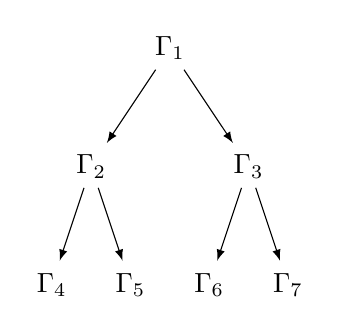
\begin{tikzpicture}[shorten >=1pt,
    edge from parent/.style={draw,-latex},
    level 1/.style={sibling distance=2cm},
    level 2/.style={sibling distance=1cm}]
    \node(){$\Gamma_1$}
    child { node{$\Gamma_2$}
        child {node{$\Gamma_4$}}
        child {node{$\Gamma_5$}}
    }
    child { node{$\Gamma_3$}
        child {node{$\Gamma_6$}}
        child {node{$\Gamma_7$}}
    }
    ;
\end{tikzpicture}

\end{center}

\underline{Example}

Let $\lambda=0$ and $K(\vec{x}, \vec{y})=\log(||\vec{x} - \vec{y}||)=\frac{1}{2}\log(||\vec{x} - \vec{y}||^2)$
and let the diagonal terms be 0. That is $K(\vec{x}, \vec{x}):= 0$. Let $\vec{x}$ be equispaced points on the five-lobed flower
\begin{equation*}
    \vec{x}(\theta) = \big(1 + 0.2 \cos (5 \theta)\big)
    \begin{bmatrix}
        \cos \theta \\
        \sin \theta
    \end{bmatrix}
    \qquad \theta \in [0, \pi)
\end{equation*}

Let's compute the $10^{-10}$ numerical ranks with $N=1024$.



\begin{center}
    \begin{tikzpicture}
    \matrix[
    matrix of math nodes,
    nodes in empty cells,
    left delimiter={[},
    right delimiter={]},
    every node/.style={
        color=OliveGreen,
        anchor=center,
        minimum size=3em,
        inner sep=0pt
        },
    ]
    (m)
    {
          &19&&&&&&\\
          19&&&&&&&\\
    &&    &19&&&&\\
    &&    19&&&&&\\
    &&&&  &19&&\\
    &&&&  19&&&\\
    &&&&&&&19\\
    &&&&&&19&\\
    };

    { \color{OliveGreen}
    \node[font=\Large]() at (m-1-3.south east){24};
    \node[font=\Large]() at (m-3-1.south east){24};
    \node[font=\Large]() at (m-5-7.south east){24};
    \node[font=\Large]() at (m-7-5.south east){24};
    \node[font=\LARGE]() at (m-2-6.south east){46};
    \node[font=\LARGE]() at (m-6-2.south east){46};
    \node[font=\LARGE]() at (m-1-5.south east){$A_{23}$};
    \draw[<-] (m-1-7) --  ++(3,0) node[fill=white] {$512 \times 512$};
    \draw[<-] (m-5-8) --  ++(2,0) node[fill=white] {$256 \times 256$};
    \draw[<-] (m-7-8) --  ++(2,0) node[fill=white] {$128 \times 128$};
    }
    \draw[red, dashed] (m-1-1.south west) -- (m-1-2.south east);
    \draw[red, dashed] (m-2-1.south west) -- (m-2-4.south east);
    \draw[red, dashed] (m-3-3.south west) -- (m-3-4.south east);
    \draw[red, dashed] (m-4-1.south west) -- (m-4-8.south east);
    \draw[red, dashed] (m-5-5.south west) -- (m-5-6.south east);
    \draw[red, dashed] (m-6-5.south west) -- (m-6-8.south east);
    \draw[red, dashed] (m-7-7.south west) -- (m-7-8.south east);

    \draw[dashed, red] (m-1-1.north east) -- (m-2-1.south east);
    \draw[dashed, red] (m-1-2.north east) -- (m-4-2.south east);
    \draw[dashed, red] (m-3-3.north east) -- (m-4-3.south east);
    \draw[dashed, red] (m-1-4.north east) -- (m-8-4.south east);
    \draw[dashed, red] (m-5-5.north east) -- (m-6-5.south east);
    \draw[dashed, red] (m-5-6.north east) -- (m-8-6.south east);
    \draw[dashed, red] (m-7-7.north east) -- (m-8-7.south east);

    \node[left=1em of m](){$A=$};
    \end{tikzpicture}

\end{center}

\begin{center}
    
\begin{tikzpicture}[
blob/.style={use Hobby shortcut, closed=true},
point/.style={circle, minimum size=2mm, inner sep=0pt, fill}
]
    \draw[blob] (0, 0) node {} ..
    (.8, -1.5) ..
    (3, -1) ..
    (6, -2.5) ..
    (8, -1) ..
    (6, 1.5) ..
    (5, 1) ..
    (4, .8) ..
    (3, 1.5) ..
    (1.2, 1.5)
    ;

    \draw[->, red, thick, font=\Large] (8, 2) node[fill=white](){$\Gamma_3$} -- (7.28, 1.28);
    \draw[->, red, thick, font=\Large] (0.5, 2.5) node[fill=white](){$\Gamma_2$} -- (1.2, 1.5);
    \draw[red, ultra thick](4.1, 0.6) -- (4.2, .9);
    \draw[red, ultra thick](3.4, -1.2) -- (3.5, -0.9);
    \draw[<-, thick, color=OliveGreen] (.5, .75) to[bend right=20] (7.8, .5);
    \draw[->, thick, color=OliveGreen] (3, -1) to[bend right=20] (3.5, 1.);
    \node[OliveGreen]() at (6, -1) {$A_{23}$};
    \draw [OliveGreen, ->] (4, -2) node[fill=white]{$A_{45}$} to[bend right=10] (3.75, -.5);

\end{tikzpicture}

\end{center}

Given $\sigma(\vec{x}_1), \ldots, \sigma(\vec{x}_N)$, the half corresponding to the points in $\Gamma_3$ are $\vec{x}_i$ with $i=I_3$. Then, computing $A_{23}\vec{\sigma}_{I_3}$ return the function

\begin{equation*}
    \sum_{j\in I_3} K(\vec{x}_i, \vec{x}_j)\sigma(\vec{x}_j) \qquad  \forall \quad i \in I_2
\end{equation*}

For these kernel matries, the rank of the blocks is independent of, or nearly independent of, the problem size $N$. However, requiring a unique SVD for each off-diagonal block is too restrictive to develop efficient methods to construct $A^{-1}$. A more efficient partitioning is a \emph{hierarchical semi-seperable} (HSS) decomposition

\begin{equation*}
    A = \begin{bmatrix}
        D_4    & A_{45} & A_{46} & A_{47} \\
        A_{54} & D_5    & A_{56} & A_{57} \\
        A_{64} & A_{65} & D_6    & A_{67} \\
        A_{74} & A_{75} & A_{76} & D_7    \\
\end{bmatrix}
\end{equation*}

An HSS decomposition writes each of the off-diagonal blocks as

\begin{equation*}
    A_{ij} = U_i \widetilde{A}_{ij} V^T_j
\end{equation*}

where $k \ll n$. The assumption we have made is that one matrix $U_i$ works for compressing $A_{ij}\forall j\neq i$. Similarly, one matrix $V_j^T$ works for compressing $A_{ij}\forall j\neq i$. That is, many of the blocks use the same left and right ``singular vectors". Note that we haven't exploited an hierarchical structure yet. Using this decomposition

\begin{equation*}
    A =
    \begin{bmatrix}
        D_4    & U_4\widetilde{A}_{45}V^T_5 & U_4\widetilde{A}_{46}V^T_6 & U_4\widetilde{A}_{47}V^T_7 \\
        U_5\widetilde{A}_{54}V^T_4 & D_5    & U_5\widetilde{A}_{56}V^T_6 & U_5\widetilde{A}_{57}V^T_7 \\
        U_6\widetilde{A}_{64}V^T_4 & U_6\widetilde{A}_{65}V^T_5 & D_6 & U_6\widetilde{A}_{67}V^T_7 \\
        U_7\widetilde{A}_{74}V^T_4 & U_7\widetilde{A}_{75}V^T_5 & U_7\widetilde{A}_{76}V^T_6 & D_7    \\
    \end{bmatrix}
\end{equation*}

%% Lecture 26

\begin{equation*}
    A =
    \begin{bmatrix}
        D_4    & & & \\
        & D_5    & & \\
        & & D_6    & \\
        & & & D_7    \\
    \end{bmatrix}
    +
    \begin{bmatrix}
        U_4    & & & \\
        & U_5    & & \\
        & & U_6    & \\
        & & & U_7    \\
    \end{bmatrix}
    \begin{bmatrix}
        0    & \widetilde{A}_{45} & \widetilde{A}_{46} & \widetilde{A}_{47} \\
        \widetilde{A}_{54} & 0 & \widetilde{A}_{56} & \widetilde{A}_{57} \\
        \widetilde{A}_{64} & \widetilde{A}_{65} & 0 & \widetilde{A}_{67} \\
        \widetilde{A}_{74} & \widetilde{A}_{75} & \widetilde{A}_{76} &    0 \\
    \end{bmatrix}
    \begin{bmatrix}
        V^T_4    & & & \\
        & V^T_5    & & \\
        & & V^T_6    & \\
        & & & V^T_7    \\
    \end{bmatrix}
\end{equation*}
\begin{center}
    
\begin{tikzpicture}
\matrix[
left delimiter = {[},
right delimiter = {]},
matrix of nodes,
every node/.style={
    draw,
    pattern=north west lines,
    minimum size=.5cm
},
row sep=1mm,
column sep=1mm
]
(D)
{
\ &&&\\
&\ &&\\
&&\ &\\
&&&\ \\
};
\node[right=1em of D](){+};
\matrix[
right=3.5em of D.north east,
anchor=north west,
left delimiter = {[},
right delimiter = {]},
matrix of nodes,
every node/.style={
    draw,
    pattern=north west lines,
    minimum height=.8cm
},
row sep=1mm,
column sep=1mm
]
(U)
{
\ &&&\\
&\ &&\\
&&\ &\\
&&&\ \\
};
\matrix[
right=2em of U.north east,
anchor=north west,
left delimiter = {[},
right delimiter = {]},
matrix of nodes,
every node/.style={
    draw,
    minimum size=2mm
},
row sep=1mm,
column sep=1mm
]
(At)
{
&\ &\ &\ \\
\ &&\ &\ \\
\ &\ &&\ \\
\ &\ &\ &\\
};
\matrix[
right=2em of At.north east,
anchor=north west,
left delimiter = {[},
right delimiter = {]},
matrix of nodes,
every node/.style={
    draw,
    pattern=north west lines,
    minimum width=.8cm
},
row sep=1mm,
column sep=1mm
]
(V)
{
\ &&&\\
&\ &&\\
&&\ &\\
&&&\ \\
};
\node[left=1em of D](){$A=$};
\node[above=1em of D, color=OliveGreen](){$4n \times 4n$};
\node[above=1em of U, color=OliveGreen](){$4n \times 4k$};
\node[below=1em of At, color=OliveGreen](){$4k \times 4k$};
\node[below=1em of V, color=OliveGreen](){$4k \times 4n$};
\end{tikzpicture}

\end{center}

\begin{equation*}
    = \qquad D \qquad + \qquad  U \qquad  \widetilde{A} \qquad V^T
\end{equation*}
This facterization is not possible if each $A_{ij}$ required a different $U_{ij}$ for each $j$ and a different $V^T_{ij}$ for each $i$. Applying the Woodbury identity
\begin{equation*}
    A^{-1} =
    \left(
    D + U \widetilde{A} V^T
    \right)^{-1}
    =
    D{-1} - D^{-1}U
    \left(
    \widetilde{A} - V^T D^{-1}U
    \right)^{-1}
    V^T D^{-1}
\end{equation*}
\begin{center}
    
\begin{tikzpicture}
\matrix[
left delimiter = {[},
right delimiter = {]},
matrix of nodes,
every node/.style={
    draw,
    minimum size=.5cm
},
row sep=1mm,
column sep=1mm
]
(D)
{
\ &&&\\
&\ &&\\
&&\ &\\
&&&\ \\
};
\node[right=1em of D](){+};
\matrix[
right=3.5em of D.north east,
anchor=north west,
left delimiter = {[},
right delimiter = {]},
matrix of nodes,
every node/.style={
    draw,
    minimum height=.8cm
},
row sep=1mm,
column sep=1mm
]
(U)
{
\ &&&\\
&\ &&\\
&&\ &\\
&&&\ \\
};
\matrix[
right=2em of U.north east,
anchor=north west,
left delimiter = {[},
right delimiter = {]},
matrix of nodes,
every node/.style={
    draw,
    minimum size=2mm
},
row sep=1mm,
column sep=1mm
]
(At)
{
\ &\ &\ &\ \\
\ &\ &\ &\ \\
\ &\ &\ &\ \\
\ &\ &\ &\ \\
};
\matrix[
right=2em of At.north east,
anchor=north west,
left delimiter = {[},
right delimiter = {]},
matrix of nodes,
every node/.style={
    draw,
    minimum width=.8cm
},
row sep=1mm,
column sep=1mm
]
(V)
{
\ &&&\\
&\ &&\\
&&\ &\\
&&&\ \\
};
\node[left=1em of D](){$A^{-1}=$};
\node[below=1em of D](){$G$};
\node[below=1em of U](){$E$};
\node[below=1em of At](){$\left(\widetilde{A}-\widetilde{D}\right)^{-1}$};
\node[below=1em of V](){$F^T$};
\end{tikzpicture}

\end{center}
where
\begin{align*}
    \widetilde{D} &= V^TD^{-1}U \\
    E &= D^{-1} \\
    F &= V^TD^{-1} \\
    G &= D^{-1}
\end{align*}
The computational cost is now 4 $n\times n$ matrix inversion and a $4k\times 4k$ matrix inverse

\begin{equation*}
    \Rightarrow \bigO{4n^3 + (4k)^3} = \bigO{4n^3 + 64k^3} = \bigO{4n^3}
\end{equation*}
Assuming $k\ll n$

In contrast, inverting the $4n\times 4n$ matrix costs
\begin{equation*}
    \bigO{(4n)^3} = \bigO{64n^3}
\end{equation*}
$\Rightarrow$ A speed up of $16\times$.

However, this can speed up even more. First, let the decompositions of
$A_{ij} = U_i \widetilde{A}_{ij}V^T_j$ be the interpolative decomposition (ID). That is, we find an index set $J$, of size $k$, of a low-rank matrix $A_{ij}$

\begin{equation*}
    A_{ij} = A_{ij}(:, J) X
\end{equation*}
where $X(:, J)=I_k$ and all entries of $X$ are bounded by 2 in absolute value. We can think of $X$ as being $V^T_j$. Applying an ID to $A^T$ gives a $U_i$.

\underline{Example}
\begin{align*}
    A_{ij} &=
    \begin{bmatrix}
        2 & 1 & 3 \\
        1 & 3 & 4 \\
        1 & 2 & 3
    \end{bmatrix}
\end{align*}
\begin{align*}
    \begin{bmatrix}
        3 \\
        4 \\
        3
    \end{bmatrix}
    &= 1\cdot
    \begin{bmatrix}
        2 \\
        1 \\
        1
    \end{bmatrix}
    + 1 \cdot
    \begin{bmatrix}
        1 \\
        3 \\
        2
    \end{bmatrix}
    \\
    \begin{bmatrix}
        1 & 2 & 3
    \end{bmatrix}
    &=
    \frac{1}{5}
    \begin{bmatrix}
        2 & 1 & 3
    \end{bmatrix}
    +
    \frac{3}{5}
    \begin{bmatrix}
        1 & 3 & 4
    \end{bmatrix}
\end{align*}
\begin{align*}
    \Rightarrow A_{ij} &=
    \begin{bmatrix}
        2 & 1 \\
        1 & 3 \\
        1 & 2
    \end{bmatrix}
    \begin{bmatrix}
        1 & 0 & 1 \\
        0 & 1 & 1
    \end{bmatrix}
    =
    \begin{bmatrix}
        1 & 0 \\
        0 & 1 \\
        1/5 & 3/5
    \end{bmatrix}
    \begin{bmatrix}
        2 & 1 \\
        1 & 3
    \end{bmatrix}
    \begin{bmatrix}
        1 & 0 & 1 \\
        0 & 1 & 1
    \end{bmatrix}\\
    &= U_i \widetilde{A}_{ij} V^T_j
\end{align*}

Note the $\widetilde{A}_{ij}$ is a submatrix of $A_{ij}$. Therefore, we only need to store index sets and the parts of $U_i$ and $V^T_j$ that are not in the index set of $J$.

Next we find a way to compress $A$. Given a vector $[f_4, f_5, f_6, f_7]^T$, finding $A^{-1}$ is equivalent to developing a method to solve
\begin{equation*}
    A
    \begin{bmatrix}
        q_4 \\
        q_5 \\
        q_6 \\
        q_7 \\
    \end{bmatrix}
    =
    \begin{bmatrix}
        f_4 \\
        f_5 \\
        f_6 \\
        f_7 \\
    \end{bmatrix}
\end{equation*}
Recall that

\begin{equation*}
    A =
    \begin{bmatrix}
        D_4    & U_4\widetilde{A}_{45}V^T_5 & U_4\widetilde{A}_{46}V^T_6 & U_4\widetilde{A}_{47}V^T_7 \\
        U_5\widetilde{A}_{54}V^T_4 & D_5    & U_5\widetilde{A}_{56}V^T_6 & U_5\widetilde{A}_{57}V^T_7 \\
        U_6\widetilde{A}_{64}V^T_4 & U_6\widetilde{A}_{65}V^T_5 & D_6 & U_6\widetilde{A}_{67}V^T_7 \\
        U_7\widetilde{A}_{74}V^T_4 & U_7\widetilde{A}_{75}V^T_5 & U_7\widetilde{A}_{76}V^T_6 & D_7    \\
    \end{bmatrix}
\end{equation*}

Introductin the extended variables $\widetilde{q}_i = V^T_i q_i$

Then, $A\vec{q} = \vec{f}$ is equivalent to the extended system

\begin{center}
    
\begin{tikzpicture}
\matrix[
right delimiter = {]},
left delimiter = {[},
matrix of math nodes,
nodes in empty cells,
every node/.style={}
]
(A)
{
$D_4$&&& & 0& $U_4\widetilde{A}_{45}$ & $U_4\widetilde{A}_{46}$ & $U_4\widetilde{A}_{47}$ \\
&$D_5$&& & $U_5\widetilde{A}_{54}$ & 0   & $U_5\widetilde{A}_{56}$ & $U_5\widetilde{A}_{57}$ \\
&&$D_6$& & $U_6\widetilde{A}_{64}$ & $U_6\widetilde{A}_{65}$ & 0 & $U_6\widetilde{A}_{67}$ \\
&&&$D_7$ & $U_7\widetilde{A}_{74}$ & $U_7\widetilde{A}_{75}$ & $U_7\widetilde{A}_{76}$ & 0    \\
$-V^T_4$&&&&$I$&&&\\
&$-V^T_5$&&&&$I$&&\\
&&$-V^T_6$&&&&$I$&\\
&&&$-V^T_7$&&&&$I$\\
};
\matrix[
right=1.5em of A,
right delimiter = {]},
left delimiter = {[},
matrix of math nodes,
nodes in empty cells,
every node/.style={
minimum height = 1.75em
}
]
(q)
{
$q_4$ \\
$q_5$ \\
$q_6$ \\
$q_7$ \\
$\widetilde{q_4}$\\
$\widetilde{q_5}$\\
$\widetilde{q_6}$\\
$\widetilde{q_7}$\\
};
\node[right=1em of q](){=};
\matrix[
right=3.5em of q,
right delimiter = {]},
left delimiter = {[},
matrix of math nodes,
nodes in empty cells,
every node/.style={
minimum height = 1.75em
}
]
(f)
{
$f_4$ \\
$f_5$ \\
$f_6$ \\
$f_7$ \\
0\\
0\\
0\\
0\\
};
\draw[red, dashed] (A-4-1.south west) -- (f-4-1.south east);
\draw[red, dashed] (A-2-5.north west)++(0, 1em) -- (A-8-4.south east);
\end{tikzpicture}

\end{center}

%% Lecture 27

We now eliminate $q_4, q_5, q_6, q_7$ using a (block) Schur complement so that we are instead solving for $\widetilde{q}_4, \widetilde{q}_5, \widetilde{q}_6, \widetilde{q}_7$

\begin{equation*}
    \Rightarrow
    \begin{bmatrix}
        D_4    & & & \\
        & D_5    & & \\
        & & D_6    & \\
        & & & D_7    \\
    \end{bmatrix}
    \begin{bmatrix}
        q_4 \\
        q_5 \\
        q_6 \\
        q_7 \\
    \end{bmatrix}
    = -
        \begin{bmatrix}
        0    & U_4\widetilde{A}_{45} & U_4\widetilde{A}_{46} & U_4\widetilde{A}_{47} \\
        U_5\widetilde{A}_{54} & 0 & U_5\widetilde{A}_{56} & U_5\widetilde{A}_{57} \\
        U_6\widetilde{A}_{64} & U_6\widetilde{A}_{65} & 0 & U_6\widetilde{A}_{67} \\
        U_7\widetilde{A}_{74} & U_7\widetilde{A}_{75} & U_7\widetilde{A}_{76} &    0 \\
    \end{bmatrix}
    \begin{bmatrix}
        \widetilde{q}_4 \\
        \widetilde{q}_5 \\
        \widetilde{q}_6 \\
        \widetilde{q}_7 \\
    \end{bmatrix}
    +
    \begin{bmatrix}
        f_4 \\
        f_5 \\
        f_6 \\
        f_7 \\
    \end{bmatrix}
\end{equation*}
\begin{align*}
    \Rightarrow
    &\begin{bmatrix}
        -V^T_4    & & & \\
        & -V^T_5    & & \\
        & & -V^T_6    & \\
        & & & -V^T_7    \\
    \end{bmatrix}
    \begin{bmatrix}
        D_4    & & & \\
        & D_5    & & \\
        & & D_6    & \\
        & & & D_7    \\
    \end{bmatrix}^{-1} \cdot
    \\
    &\left(
    -
    \begin{bmatrix}
    0    & U_4\widetilde{A}_{45} & U_4\widetilde{A}_{46} & U_4\widetilde{A}_{47} \\
    U_5\widetilde{A}_{54} & 0 & U_5\widetilde{A}_{56} & U_5\widetilde{A}_{57} \\
    U_6\widetilde{A}_{64} & U_6\widetilde{A}_{65} & 0 & U_6\widetilde{A}_{67} \\
    U_7\widetilde{A}_{74} & U_7\widetilde{A}_{75} & U_7\widetilde{A}_{76} &    0 \\
\end{bmatrix}
\begin{bmatrix}
    \widetilde{q}_4 \\
    \widetilde{q}_5 \\
    \widetilde{q}_6 \\
    \widetilde{q}_7 \\
\end{bmatrix}
+
\begin{bmatrix}
    f_4 \\
    f_5 \\
    f_6 \\
    f_7 \\
\end{bmatrix}
    \right)
    + I
\begin{bmatrix}
    \widetilde{q}_4 \\
    \widetilde{q}_5 \\
    \widetilde{q}_6 \\
    \widetilde{q}_7 \\
\end{bmatrix}
=
\begin{bmatrix}
    0 \\
    0 \\
    0 \\
    0 \\
\end{bmatrix}
\end{align*}
%
\begin{align*}
    \Rightarrow
    &
    \begin{bmatrix}
        V^T_4D_4^{-1}    & & & \\
        & V^T_5D_5^{-1}    & & \\
        & & V^T_6D_6^{-1}    & \\
        & & & V^T_7D_7^{-1}    \\
    \end{bmatrix}
\begin{bmatrix}
    0    & U_4\widetilde{A}_{45} & U_4\widetilde{A}_{46} & U_4\widetilde{A}_{47} \\
    U_5\widetilde{A}_{54} & 0 & U_5\widetilde{A}_{56} & U_5\widetilde{A}_{57} \\
    U_6\widetilde{A}_{64} & U_6\widetilde{A}_{65} & 0 & U_6\widetilde{A}_{67} \\
    U_7\widetilde{A}_{74} & U_7\widetilde{A}_{75} & U_7\widetilde{A}_{76} &    0 \\
\end{bmatrix}
\cdot
\\
&
\begin{bmatrix}
    \widetilde{q}_4 \\
    \widetilde{q}_5 \\
    \widetilde{q}_6 \\
    \widetilde{q}_7 \\
\end{bmatrix}
+
\begin{bmatrix}
    \widetilde{q}_4 \\
    \widetilde{q}_5 \\
    \widetilde{q}_6 \\
    \widetilde{q}_7 \\
\end{bmatrix}
=
\begin{bmatrix}
    V^T_4D_4^{-1}f_4 \\
    V^T_5D_5^{-1}f_5 \\
    V^T_6D_6^{-1}f_6 \\
    V^T_7D_7^{-1}f_7 \\
\end{bmatrix}
\end{align*}

\begin{equation*}
    \Rightarrow
\begin{bmatrix}
    I    & V^T_4D_4^{-1}U_4\widetilde{A}_{45} & V^T_4D_4^{-1}U_4\widetilde{A}_{46} & V^T_4D_4^{-1}U_4\widetilde{A}_{47} \\
    V^T_5D_5^{-1}U_5\widetilde{A}_{54} & I & V^T_5D_5^{-1}U_5\widetilde{A}_{56} & V^T_5D_5^{-1}U_5\widetilde{A}_{57} \\
    V^T_6D_6^{-1}U_6\widetilde{A}_{64} & V^T_6D_6^{-1}U_6\widetilde{A}_{65} & I & V^T_6D_6^{-1}U_6\widetilde{A}_{67} \\
    V^T_7D_7^{-1}U_7\widetilde{A}_{74} & V^T_7D_7^{-1}U_7\widetilde{A}_{75} & V^T_7D_7^{-1}U_7\widetilde{A}_{76} &    I \\
\end{bmatrix}
\begin{bmatrix}
    \widetilde{q}_4 \\
    \widetilde{q}_5 \\
    \widetilde{q}_6 \\
    \widetilde{q}_7 \\
\end{bmatrix}
=
\begin{bmatrix}
    V^T_4D_4^{-1}f_4 \\
    V^T_5D_5^{-1}f_5 \\
    V^T_6D_6^{-1}f_6 \\
    V^T_7D_7^{-1}f_7 \\
\end{bmatrix}
\end{equation*}

We have defined $\widetilde{A}_{ij}$ for $i \neq j$, but not $\widetilde{A}_{ii}$.

We let

\begin{equation*}
    \widetilde{A}_{ii} = (V^T_i D_i^{-1}U_i)^{-1}
\end{equation*}
Multiplying each row by  $\widetilde{A}_{ii}$, we have
\begin{equation*}
        \begin{bmatrix}
        \widetilde{A}_{44}    & \widetilde{A}_{45} & \widetilde{A}_{46} & \widetilde{A}_{47} \\
        \widetilde{A}_{54} & \widetilde{A}_{55}     & \widetilde{A}_{56} & \widetilde{A}_{57} \\
        \widetilde{A}_{64} & \widetilde{A}_{65} & \widetilde{A}_{66}     & \widetilde{A}_{67} \\
        \widetilde{A}_{74} & \widetilde{A}_{75} & \widetilde{A}_{76} &    \widetilde{A}_{77}     \\
    \end{bmatrix}
    \begin{bmatrix}
        \widetilde{q}_4 \\
        \widetilde{q}_5 \\
        \widetilde{q}_6 \\
        \widetilde{q}_7 \\
    \end{bmatrix}
    =
    \begin{bmatrix}
        \widetilde{f}_4 \\
        \widetilde{f}_5 \\
        \widetilde{f}_6 \\
        \widetilde{f}_7 \\
    \end{bmatrix}
\end{equation*}
where $\widetilde{f}_i = \widetilde{A}_{ii}V^T_iD_i^{-1}f_i$.

This is now a $4k \times 4k$ matrix for $\widetilde{q}_i$ instead of a $4n \times 4n$ matrix for $q_i$. Moreover, each off-diagonal block is simply a submatrix of the full matrix $A$. The speed up is $(\frac{n}{k})^3$. To get an asymtotically faster scheme, we recurse.


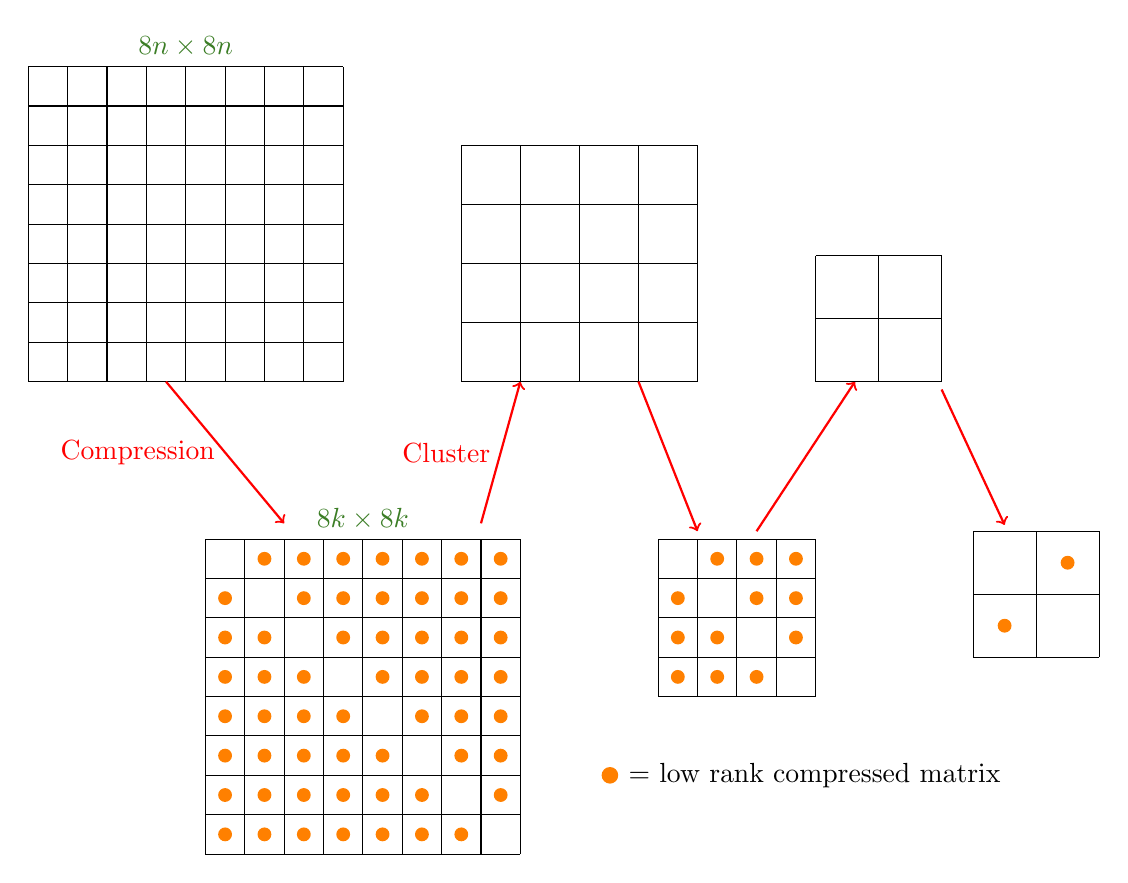
\begin{tikzpicture}

%% Step 1
\begin{scope}[]
    \draw[step=0.5] (0, 0) grid (4, 4);
    \node[OliveGreen]() at (2, 4.25){$8n\times 8n$};
\end{scope}

%% Step 2
\begin{scope}[
xshift = 2.25cm,
yshift = -6cm
]
    \draw[step=0.5] (0, 0) grid (4, 4);
    \node[OliveGreen]() at (2, 4.25){$8k\times 8k$};
    \draw[->, red, thick] (-0.5, 6) -- node[left]{Compression} (1, 4.2);
    \draw[->, red, thick] (3.5, 4.2) -- node[left]{Cluster} (4, 6);

    \foreach \i in {0.25, .75, ..., 3.75}{
        \foreach \j in {0.25, 0.75, ..., 3.75}{
        \node[inner sep=0pt, minimum size=5pt, fill, orange, circle]  () at (\i, \j) {};
        };
    };

    \foreach \i/\j in {
0.25/3.75,
0.75/3.25,
1.25/2.75,
1.75/2.25,
2.25/1.75,
2.75/1.25,
3.25/0.75,
3.75/0.25
    }{
        \node[inner sep=0pt, minimum size=6pt, fill, white]  () at (\i, \j) {};
    };
\end{scope}

%% Step 3
\begin{scope}[
xshift = 5.5cm,
scale=0.75
]
    \draw[step=1] (0, 0) grid (4, 4);
\end{scope}

%% Step 4
\begin{scope}[
xshift = 8cm,
yshift = -4cm,
scale=0.5
]
    \draw[step=1] (0, 0) grid (4, 4);
    \draw[->, red, thick] (-0.5, 8) -- (1, 4.2);
    \draw[->, red, thick] (2.5, 4.2) -- (5, 8);
    \foreach \i in {0.5, 1.5, ..., 3.75}{
        \foreach \j in {0.5, 1.5, ..., 3.75}{
        \node[inner sep=0pt, minimum size=5pt, fill, orange, circle]  () at (\i, \j) {};
        };
    };

    \foreach \i/\j in {
0.5/3.5,
1.5/2.5,
2.5/1.5,
3.5/0.5
    }{
        \node[inner sep=0pt, minimum size=6pt, fill, white]  () at (\i, \j) {};
    };
\end{scope}


%% Step 5
\begin{scope}[
xshift = 10cm,
scale=0.4
]
    \draw[step=2] (0, 0) grid (4, 4);
\end{scope}

%% Step 6
\begin{scope}[
xshift = 12cm,
yshift = -3.5cm,
scale=0.4
]
    \draw[step=2] (0, 0) grid (4, 4);
    \draw[->, red, thick] (-1, 8.5) -- (1, 4.2);
        \foreach \i in {1, 3, ..., 3.75}{
        \foreach \j in {1, 3, ..., 3.75}{
        \node[inner sep=0pt, minimum size=5pt, fill, orange, circle]  () at (\i, \j) {};
        };
    };
\foreach \i/\j in {
1/3, 3/1
    }{
        \node[inner sep=0pt, minimum size=6pt, fill, white]  () at (\i, \j) {};
    };
\end{scope}
\node[xshift=7.5cm, yshift=-5cm, right] () {= low rank compressed matrix};
\node[inner sep=0pt, left, minimum size=6pt, fill, orange, circle]  () at (7.5cm, -5cm) {};
\end{tikzpicture}


The only matricies in theis decomposition that are new are the diagonal blocks. All other blocks are submatrices of the original coefficient matrix since we are using the ID.

%% Lecture 28

In matrix form, we have constructed the following telescoping factorization

\begin{align*}
    A = U^{(3)}
    \left( U^{(2)}
        \left( U^{(1)} B^{(0)} V^{(1)T} + B^{(1)} \right)
        V^{(2)T} +B^{(2)}
    \right)V^{(3)T} + D^{(3)}
\end{align*}



\begin{center}
    
    \begin{tikzpicture}[
    ]
        \matrix
        [U matrix]
        (U3)
        {
        \ &&&&&&&\\
        &\ &&&&&&\\
        &&\ &&&&&\\
        &&&\ &&&&\\
        &&&&\ &&&\\
        &&&&&\ &&\\
        &&&&&&\ &\\
        &&&&&&&\ \\
        };
        \node[left = 1em of U3](){=};
        \matrix
        [U matrix,
        right=3em of U3.north east,
        anchor=north west, ]
        (U2)
        {
        \ &&&\\
        &\ &&\\
        &&\ &\\
        &&&\ \\
        };

        \draw[thick] (U2-1-1.north west)++(-1em, 1em) to[bend right=15] ++(0, -9em);

        \matrix
        [U matrix,
        right=2em of U2.north east,
        anchor=north west, ]
        (U1)
        {
        \ &\\
        &\ \\
        };

        \draw[thick] (U1-1-1.north west)++(-1em, 1em) to[bend right=15] ++(0, -5em);

        \matrix
        [B matrix,
        right=2em of U1.north east,
        anchor=north west, ]
        (B0)
        {
        \ &\\
        &\ \\
        };
        \matrix
        [V matrix,
        right=2em of B0.north east,
        anchor=north west, ]
        (V1)
        {
        \ &\\
        &\ \\
        };
        \node[right=1em of V1](){+};

        \node[OliveGreen, right=2em of U3-2-2](){$U^{(3)}$};
        \node[OliveGreen, right=1em of U2-1-1](){$U^{(2)}$};
        \node[OliveGreen, below=.5em of U1](){$U^{(1)}$};
        \node[OliveGreen, below=.5em of B0](){$B^{(0)}$};
        \node[OliveGreen, below=.5em of V1](){$V^{(1)T}$};
    \end{tikzpicture}

\end{center}

\begin{center}
    
    \begin{tikzpicture}[ ]
    \matrix
        [B matrix,  ]
        (B1)
        {
        &\ &&\\
        \ &&&\\
        &&&\ \\
        &&\ &\\
        };

    \node[OliveGreen, right=.25em of B1-1-2](){$B^{(1)}$};
    \draw[thick] (B1-1-2.north east)++(3.2em, .5em) to[bend left=15] ++(0, -5em);

    \matrix
        [V matrix, right=2em of B1.north east, anchor=north west]
        (V2)
        {
        \ &&&\\
        &\ &&\\
        &&\ &\\
        &&&\ \\
        };
        \node[OliveGreen, right=2em of V2-1-1](){$V^{(2)T}$};
        \node[right=1em of V2](){+};
        \matrix[B matrix, right=3em of V2.north east, anchor=north west]
        (B2)
        {
        &\ &&&&&&\\
        \ &&&&&&&\\
        &&&\ &&&&\\
        &&\ &&&&&\\
        &&&&&\ &&\\
        &&&\ &&&&\\
        &&&&&&&\ \\
        &&&&&&\ &\\
        };
        \draw[thick] (B2-1-2.north east)++(7em, 1em) to[bend left=15] ++(0, -9em);
        \node[OliveGreen, right=2em of B2-1-2](){$B^{(2)}$};
        \node[right=2em of B2](){$\times$};
    \end{tikzpicture}

\end{center}

\begin{center}
    
    \begin{tikzpicture}[ ]
    \matrix
        [V matrix, ]
        (V3)
        {
        \ &&&&&&&\\
        &\ &&&&&&\\
        &&\ &&&&&\\
        &&&\ &&&&\\
        &&&&\ &&&\\
        &&&&&\ &&\\
        &&&&&&\ &\\
        &&&&&&&\ \\
        };
        \node[right=1em of V3](){+};

        \node[OliveGreen, right=5em of V3-1-1](){$V^{(3)T}$};
    \matrix[B matrix, right=3em of V3.north east, anchor=north west]
        (D3)
        {
        \ &&&&&&&\\
        &\ &&&&&&\\
        &&\ &&&&&\\
        &&&\ &&&&\\
        &&&&\ &&&\\
        &&&&&\ &&\\
        &&&&&&\ &\\
        &&&&&&&\ \\
        };
        \node[OliveGreen, right=3em of D3-1-1](){$D^{(3)}$};
    \end{tikzpicture}

\end{center}


Using our definitions of $E$, $F$, and $\widetilde{D}$ from two Fridays ago (March 15), after applying the Woodbury identity, we have

\begin{equation*}
    A^{-1} = E^{(3)}
    \left(
        E^{(2)}
        \left(
            E^{(1)} \widetilde{D}^{(0)} F^{(1)T}
            + \widetilde{D}^{(1)}
        \right) F^{(2)T} + \widetilde{D}^{(2)}
    \right) F^{(3)T} + \widetilde{D}^{(3)}
\end{equation*}

The only non-block diagonal matrix is $\widetilde{D}^{(0)}$
, but it is small, so can be computed directly.

This inversion can be written with fairly simple pseudocode. Recall that we are partitioning $A$ into blocks corresponding to a tree structure applied to our index set $\{ 1, \ldots, n \} = I_1$


\begin{center}
    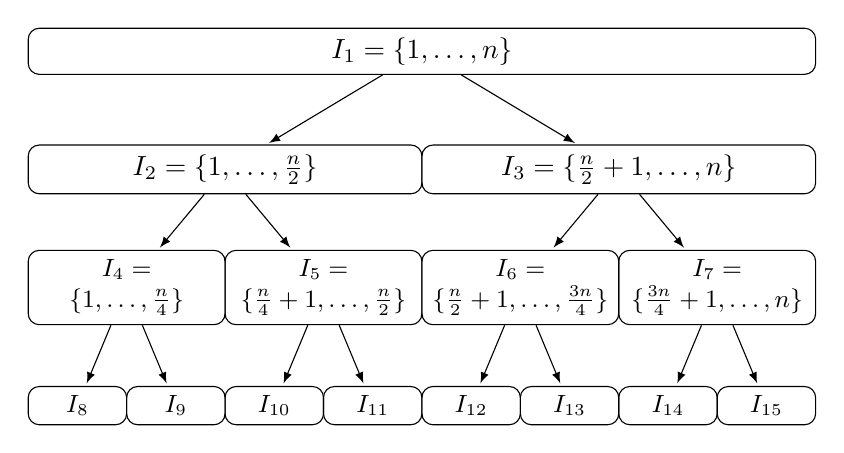
\begin{tikzpicture}[shorten >=1pt,
    edge from parent/.style={draw,-latex},
    level 1/.style={sibling distance=5cm, minimum width=5cm},
    level 2/.style={sibling distance=2.5cm, minimum width=2.5cm,font=\small},
    level 3/.style={sibling distance=1.25cm, minimum width=1.25cm},
    every node/.style = {shape=rectangle, rounded corners,
    draw, align=center}]
    \node[minimum width=10cm](I1){$I_1 = \{1, \ldots, n\}$}
    child {node{$I_2 = \{1, \ldots, \frac{n}{2}\}$}
        child{node{$I_4=$\\$\{1, \ldots, \frac{n}{4}\}$}
            child{node{$I_8$}}
            child{node{$I_9$}}
        }
        child{node{$I_5=$\\$\{\frac{n}{4}+1, \ldots, \frac{n}{2}\}$}
            child{node{$I_{10}$}}
            child{node{$I_{11}$}}
        }
    }
    child {node{$I_3 = \{\frac{n}{2}+1, \ldots, n\}$}
        child{node{$I_6=$\\$\{\frac{n}{2}+1, \ldots, \frac{3n}{4}\}$}
            child{node{$I_{12}$}}
            child{node{$I_{13}$}}
        }
        child{node{$I_7=$\\$\{ \frac{3n}{4}+1, \ldots, n\}$}
            child{node{$I_{14}$}}
            child{node{$I_{15}$}}
        }
    }
    ;
\end{tikzpicture}

\end{center}

We define all elements of the tree with no descendents as a leaf. Other nodes are called parent nodes. For each leaf node, we define,

\begin{tabular}{ccl}
    \underline{Notation} & \underline{Size} &
    \underline{Role}\\
    $D_{\tau}$ & $n \times n$ & Diagonal block of $A(I_{\tau}, I_{\tau})$ \\
    $U_{\tau}$ & $n \times k$ & Basis for the columns of the blocks in row $\tau$\\
    $V_{\tau}$ & $n \times k$ & Basis for the rowa of the blocks in column $\tau$\\
\end{tabular}

For each parent node:

\begin{tabular}{ccl}
    \underline{Notation} & \underline{Size} &
    \underline{Role}\\
    $B_{\tau}$ & $2k \times 2k$ & Interaction between the children of $\tau$\\
    $U_{\tau}$ & $2k \times k$ & Basis for the columns of the blocks in row $\tau$\\
    $V_{\tau}$ & $2k \times k$ & Basis for the rowa of the blocks in column $\tau$\\
\end{tabular}


Then, the pseudocode to compute $A^{-1}$ where $A$ is an HSS matrix is:
\begin{algorithm}[H]
    \begin{algorithmic}
    \FOR{$l = L, L-1, \ldots, 1$}
        \FOR{$\tau$ at level $l$}
            \IF {$\tau$ is a leaf node}
                \STATE $X=D_{\tau}$
            \ELSE
                \STATE Let $\sigma_1$, $\sigma_2$ be $\tau$'s children
                \STATE \begin{equation*}
                    X = \begin{bmatrix}
                        D_{\sigma_1}  & B_{\sigma_1, \sigma_2} \\
                        B_{\sigma_2, \sigma_1} & D_{\sigma_2}
                \end{bmatrix}
            \end{equation*}
            \ENDIF
            \STATE $\widetilde{D}_{\tau} = \left( V^T_{\tau}X^{-1} U_{\tau}\right)^{-1}$
            \STATE $E_{\tau} = X^{-1}  U_{\tau} D_{\tau}$
            \STATE $F^T_{\tau} = D_{\tau} V^T_{\tau}X^{-1}$
            \STATE $G_{\tau} = X^{-1} - X^{-1}U_{\tau}D_{\tau} V^T_{\tau}X^{-1}$
        \ENDFOR
    \ENDFOR
    \STATE  \begin{equation*}
        G_1 =
        \begin{bmatrix}
            D_2 & B_{23}\\
            B_{32} & D_3
        \end{bmatrix}^{-1}
\end{equation*}
      \end{algorithmic}
  \end{algorithm}

Then, $G_1$ is the inverse of $A$ with some percision stored in a compressed format. Once all these matricies are constructed and compressed, it is very fast to apply $G_1$ to lots of vectors $\vec{b}$.

